\documentclass[xetex]{beamer}

\mode<presentation> {
  \usetheme{Frankfurt}
  \setbeamercovered{transparent}
}

\usepackage{xunicode}
\usepackage{xltxtra}
\usepackage[czech]{babel}
\usepackage{palatino}
\usepackage{graphicx}
\usepackage{textpos}

\usepackage{listings}
\lstset{language=bash,
        numbers=left,
        numberstyle=\tiny,
        showstringspaces=false,
        aboveskip=-40pt,
        frame=leftline
        }

\title{Bitcoin}

\author{Karel Bílek\\Ondřej Profant}
\institute[Piráti]{Česká pirátská strana}
\date{\today}

\begin{document}

\begin{frame}
	\begin{textblock*}{0cm}(-1cm,-3.78cm)
  
\includegraphics[scale=0.6]{images/intro.jpg}
  \end{textblock*}
\end{frame}

\begin{frame}
  \titlepage
\end{frame}

\begin{frame}
  \frametitle{Osnova}
  \tableofcontents
\end{frame}	

\begin{frame}
	\frametitle{Disclaimer}
	Bitcoin je poměrně složité téma, proto není lehké připravit prezentaci, která by nepůsobila poněkud chaoticky
	a~přesto nemusela zjednodušovat.

	\bigskip

	Předem se proto omlouváme za podobné nedostatky přednášky.

	\bigskip

	Pokud máte konstruktivní připomínky či dokonce konkrétní nápady, jak prezentaci vylepšit, tak kontaktujte autory, či rovnou pošlete pull request na Githubu.
\end{frame}

\section{Měna}

\begin{frame}
	\frametitle{Měna}
	Je prostředkem směny.

	\bigskip

	Zlatý standart postupně opuštěn v průběhu 20. stol.

	Dnešní měny nejsou příliš kryty - jedná se spíše o důvěru, než o trvalou hodnotu.
\end{frame}

\section{Základní charakteristika}

\begin{frame}
	\frametitle{Základní charakteristika}

	Co je Bitcoin?
	\begin{itemize}
		\item<1-4> měna
		\item<2-4> \textbf{crypto}měna
		\item<3-4> \textbf{decentralizovaná} cryptoměna
		\item<4-4> decentralizovaná \textbf{cyber}cryptoměna
	\end{itemize}
\end{frame}

\begin{frame}
 	\frametitle{Základní charakteristika}
	\begin{itemize}
		\item bezpečná: podložena výpočetním výkonem (šifry)
		\item globální: velmi nízké poplatky za libovolnou transakci 
		\item volnost: každý může mít zdarma neomezený počet peněženek
		\item anonymita: resp. pseudoanonymita
		\item transparentí: všechny transakce jsou veřejné
		\item předem dané množství Bitcoinů $\Rightarrow$ deflační měna (?)
	\end{itemize}
\end{frame}

\section{Využití}

\begin{frame}
        \frametitle{Co lze za Bitcoin koupit}
        \begin{itemize}
                \item VPS (virtual private network)
                \item připojení k internetu
                \item HardWare (např. i na těžení Bitocinu)
		\item jidlo (např. pražský hackerspace Brmlab)
                \item sázet v kasinu (známé je Satoshi Dice)
                \item drogy etc. (např. Silk Road)
		\item \ldots{}
        \end{itemize}
\end{frame}

\begin{frame}
	\frametitle{Hedvábná stezka}
	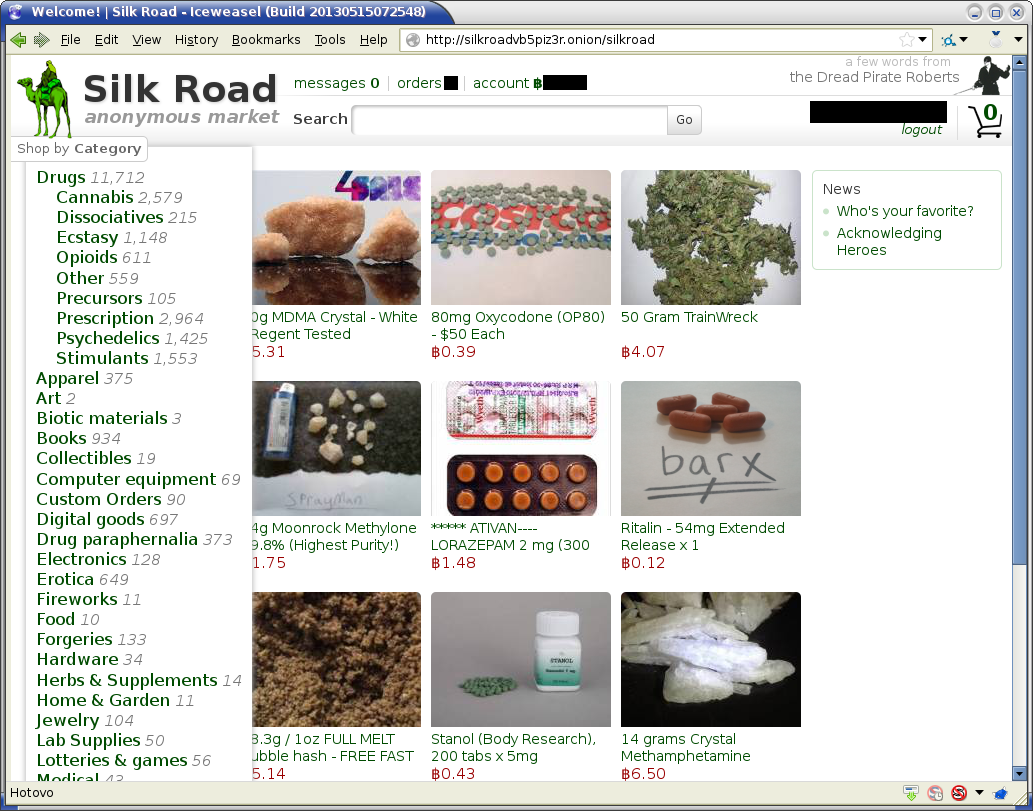
\includegraphics[scale=0.4]{images/silkroad.png}
\end{frame}

\begin{frame}
	\frametitle{Armory}
	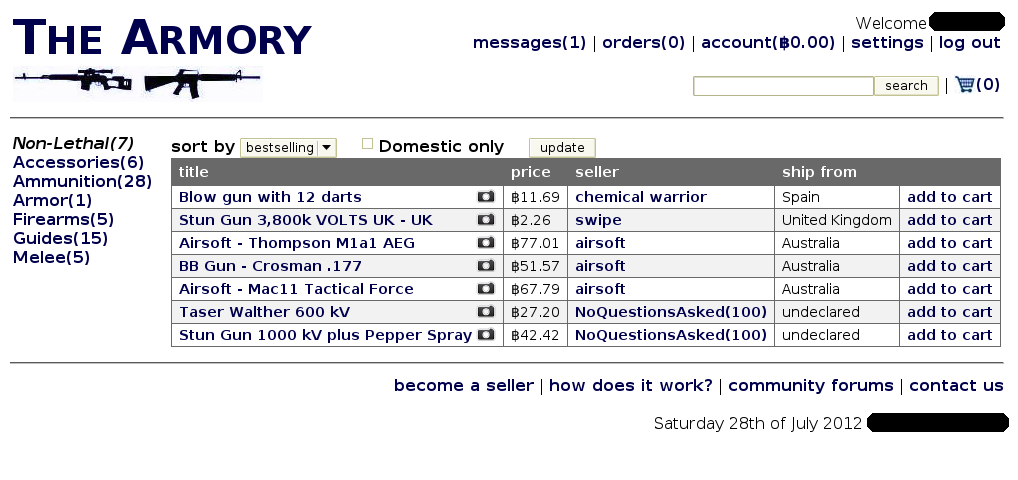
\includegraphics[scale=0.4]{images/armory.png}
\end{frame}

\begin{frame}
	\frametitle{Legalita BTC}
	Červenec 2013 zákaz v Thajsku
	%TODO
\end{frame}

\section{Historie}

\begin{frame}
  \frametitle{Historie}
        \begin{itemize}
                \item srpen 2008: registrována doména bitcoin.org
                \item říjen 2008: Bitcoin design paper published
                \item listopad 2008: Bitcoin project registered at SourceForge.net
                \item leden 2009: First Bitcoin transaction, in block 170 - from Satoshi to Hal Finney
                \item květen 2010: laszlo first to buy pizza with Bitcoins agreeing upon paying 10,000 BTC for ~\$25 worth of pizza courtesy of jercos
		\item únor 2011 parita s dolarem dle Mt.Gox
		\item květen 2013 BTC v kurzu (dle Mt.Gox) až \$220/BTC
		\item červenec 2013 prodej Satoshi Dice (Bitcoin kasino) prodáno za 126,315 BTC (cca \$11.47 million)
	\end{itemize}

        Více na: \url{https://en.bitcoin.it/wiki/History}
\end{frame}

\begin{frame}
        \frametitle{Kurz}
        Vývoj kurzu červen 2011 až květen 2014:

        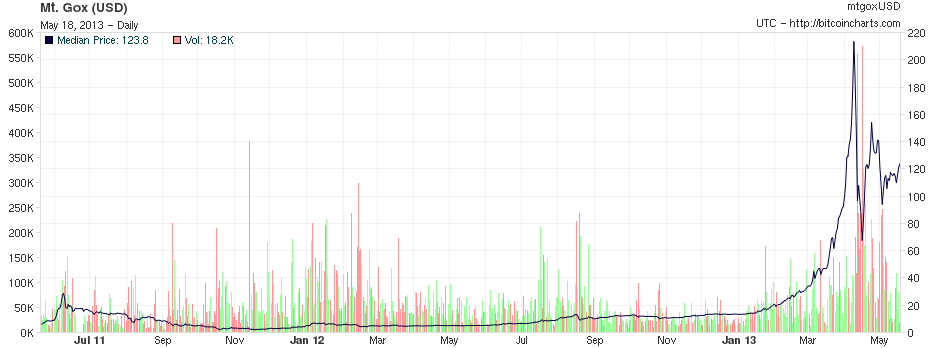
\includegraphics[scale=0.35]{images/bitcoin-exchange-rate.png}
\end{frame}


\section{Praktické použití}

\begin{frame}
	\frametitle{Praktické použití}
	Adresa je hash, např: 19bRk3XRrAfeE1Z1zr1C9M8n7d1PygHDYZ

	\bigskip

	Před provedením transakce určíme poplatek (fee). Lze i 0. Výše poplatku ovlivní rychlost potvrzení transakce (čili rychlost směny). 
\end{frame}

\begin{frame}
 \frametitle{Praktické použití - klient / peněženka}
	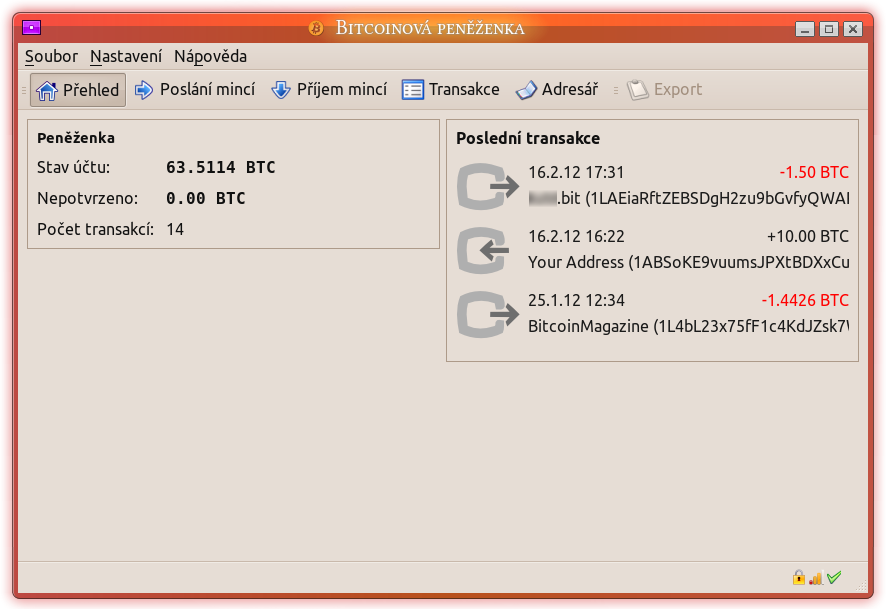
\includegraphics[scale=0.3]{images/klient.png}

	\smallskip

	Klient uchovává vaše bitcoiny, komunikuje se sítí, zobrazí vám historii plateb a umožňuje vám provádět platby nové.
\end{frame}

\begin{frame}
 \frametitle{Praktické použití}
	
	První spuštění klienta

	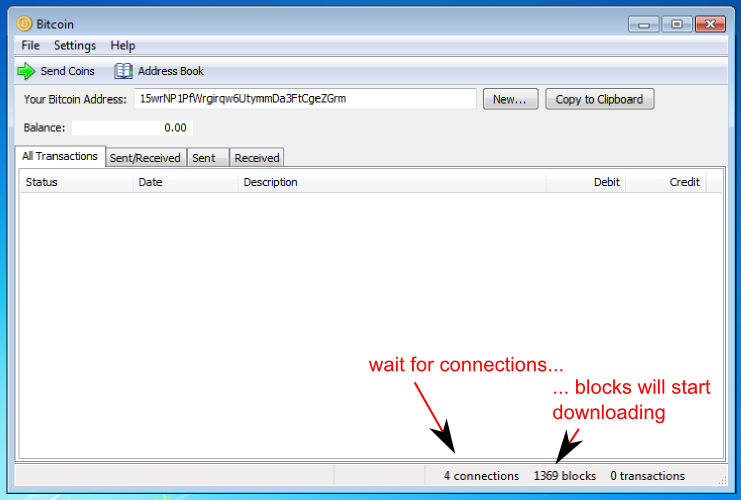
\includegraphics[scale=0.4]{images/first-time-run.png}
\end{frame}

\begin{frame}
\frametitle{Praktické použití - transakce}
	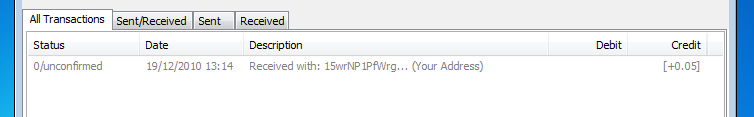
\includegraphics[scale=0.6]{images/btc-recv.png}

	\medskip        

	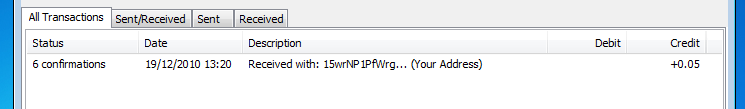
\includegraphics[scale=0.6]{images/btc-recv-confirm.png}
\end{frame}

\section{Čím je měna podložena}

\begin{frame}
        \frametitle{Způsob emitování pěnez}
        Bitcoinů je předem daný přesný počet.
        Uvolňovány jsou postupně.

        Emitování nových peněz probíhá formou odměny minerům. Tato odměna se snižuje.

        \smallskip

        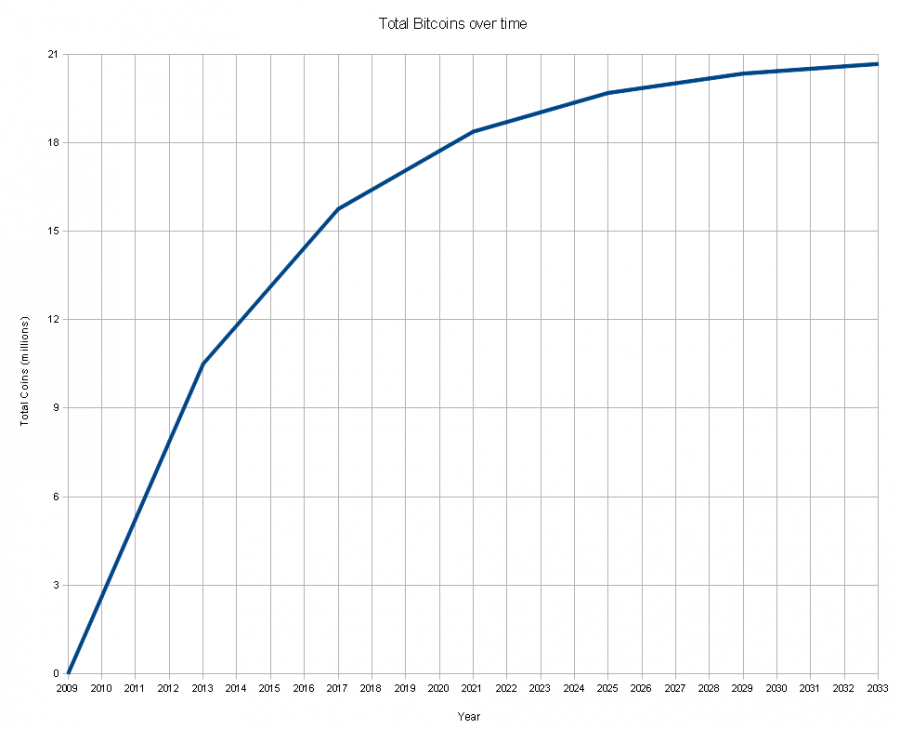
\includegraphics[scale=0.20]{images/emitation.png}
\end{frame}


\begin{frame}
	\frametitle{Čím je měna podložena}

	Blockchain je vícenásobně zahashovaná historie všech transakcí. 

	\bigskip

	Když provedeme transakci, tak se přidá do blockchainu. 

	\bigskip

	Mineři pátrají po hashy, který ho splňuje.
\end{frame}

\begin{frame}
	\frametitle{Odbočka: hash}
	
	\begin{block}{Definice}
	Hašovací funkce je matematická funkce (resp. algoritmus) pro převod vstupních dat do (relativně) malého čísla. Výstup hašovací funkce se označuje výtah, miniatura, otisk, fingerprint či hash (česky též někdy jako haš).
	\end{block}

	\bigskip

	Stručně laicky: Hash převede libovolná data (text) na text pevně dané délky. 

	\bigskip

	Převod text $\rightarrow$ hash je rychlý. Opačně je náročný (je třeba zkoušet kombinace).

\end{frame}

\begin{frame}
	\frametitle{Čím je měna podložena}
	Miner (těžař) je osoba, která řeší umělý problém zpětného odhalení hashe.

	\bigskip

	Celkově se tím do sítě Bitcoinů dostává ohromný výpočetní výkon. Který snad garantuje dostatečnou jedinečnost.

	\bigskip

	Pokud by někdo vlastnit nadpolovičný výkon, tak by se mu mohlo podařit potvrzovat neoprávněné transakce (avšak nikoliv zrušit staré - na to by byl potřeba ještě větší výkon).

	\bigskip

	Za svou snahu dostávají mineři dvě odměny (vždy za vypočítaný blok):
	\begin{itemize}
		\item fee (poplatek) z~transakcí
		\item nově uvolněné peníze (odměnu)
	\end{itemize}
\end{frame}

\begin{frame}
	\frametitle{Čím je měna podložena - podrobněji}
	\begin{enumerate}
		\item Miner vezme nezapočítané (neověřené) transakce. Vybrat si může libovolné (např. dle výše poplatku)
		\item Následně přidá ,,sůl'' (\textit{nonce}) a zkusí zda je jeho hash menší než \textit{cíl}
		\item Pokud je menší, tak svůj objev zveřejní (a tím transakce potvrdil)
			
			Pokud není menší, tak zkouší dále.¨
	\end{enumerate}

	Target/cíl/limit se každých 14 dní mění, aby průměrná délka nalezení byla 10 minut. Více na:\\
	\begin{scriptsize}
	\url{http://www.abclinuxu.cz/clanky/decentralizovana-kryptomena-bitcoin}\\
	\url{http://cs.wikipedia.org/wiki/Bitcoin}
	\end{scriptsize}
\end{frame}

\begin{frame}
	\frametitle{Čím je měna podložena}
	Těžba je dnes již extrémně náročná. 

	\bigskip

	Rozhodně se nevyplatí na procesoru. Je potřeba výkoná grafická karta (navíc AMD). Rozšiřují se specializované stroje.

	\bigskip 

	I proto se mineři raději spojují do poolů (guild, skupin, spolků).
\end{frame}

\begin{frame}
	\frametitle{Čím je měna podložena}
	
	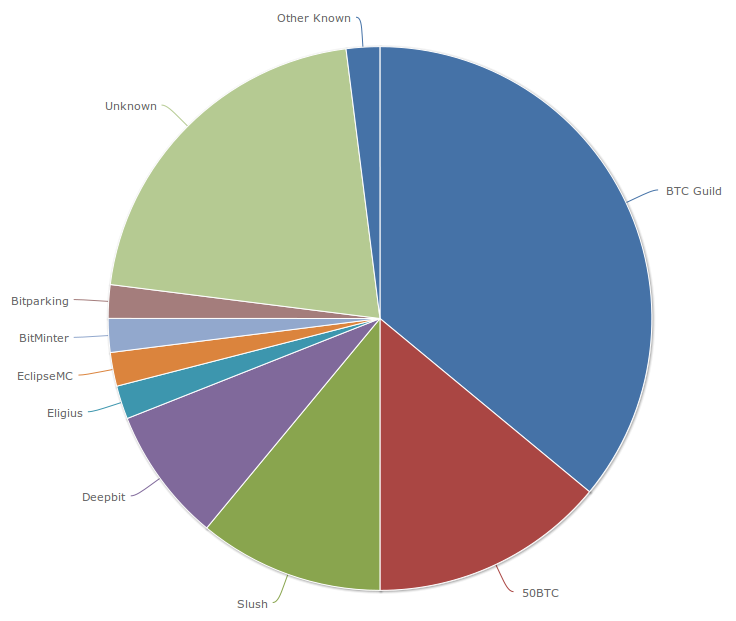
\includegraphics[scale=0.25]{images/bitcoin-pools.png}

	Přelom března/dubna 2013.

	Zdroj: \url{http://blockchain.info/pools}
\end{frame}


\begin{frame}
	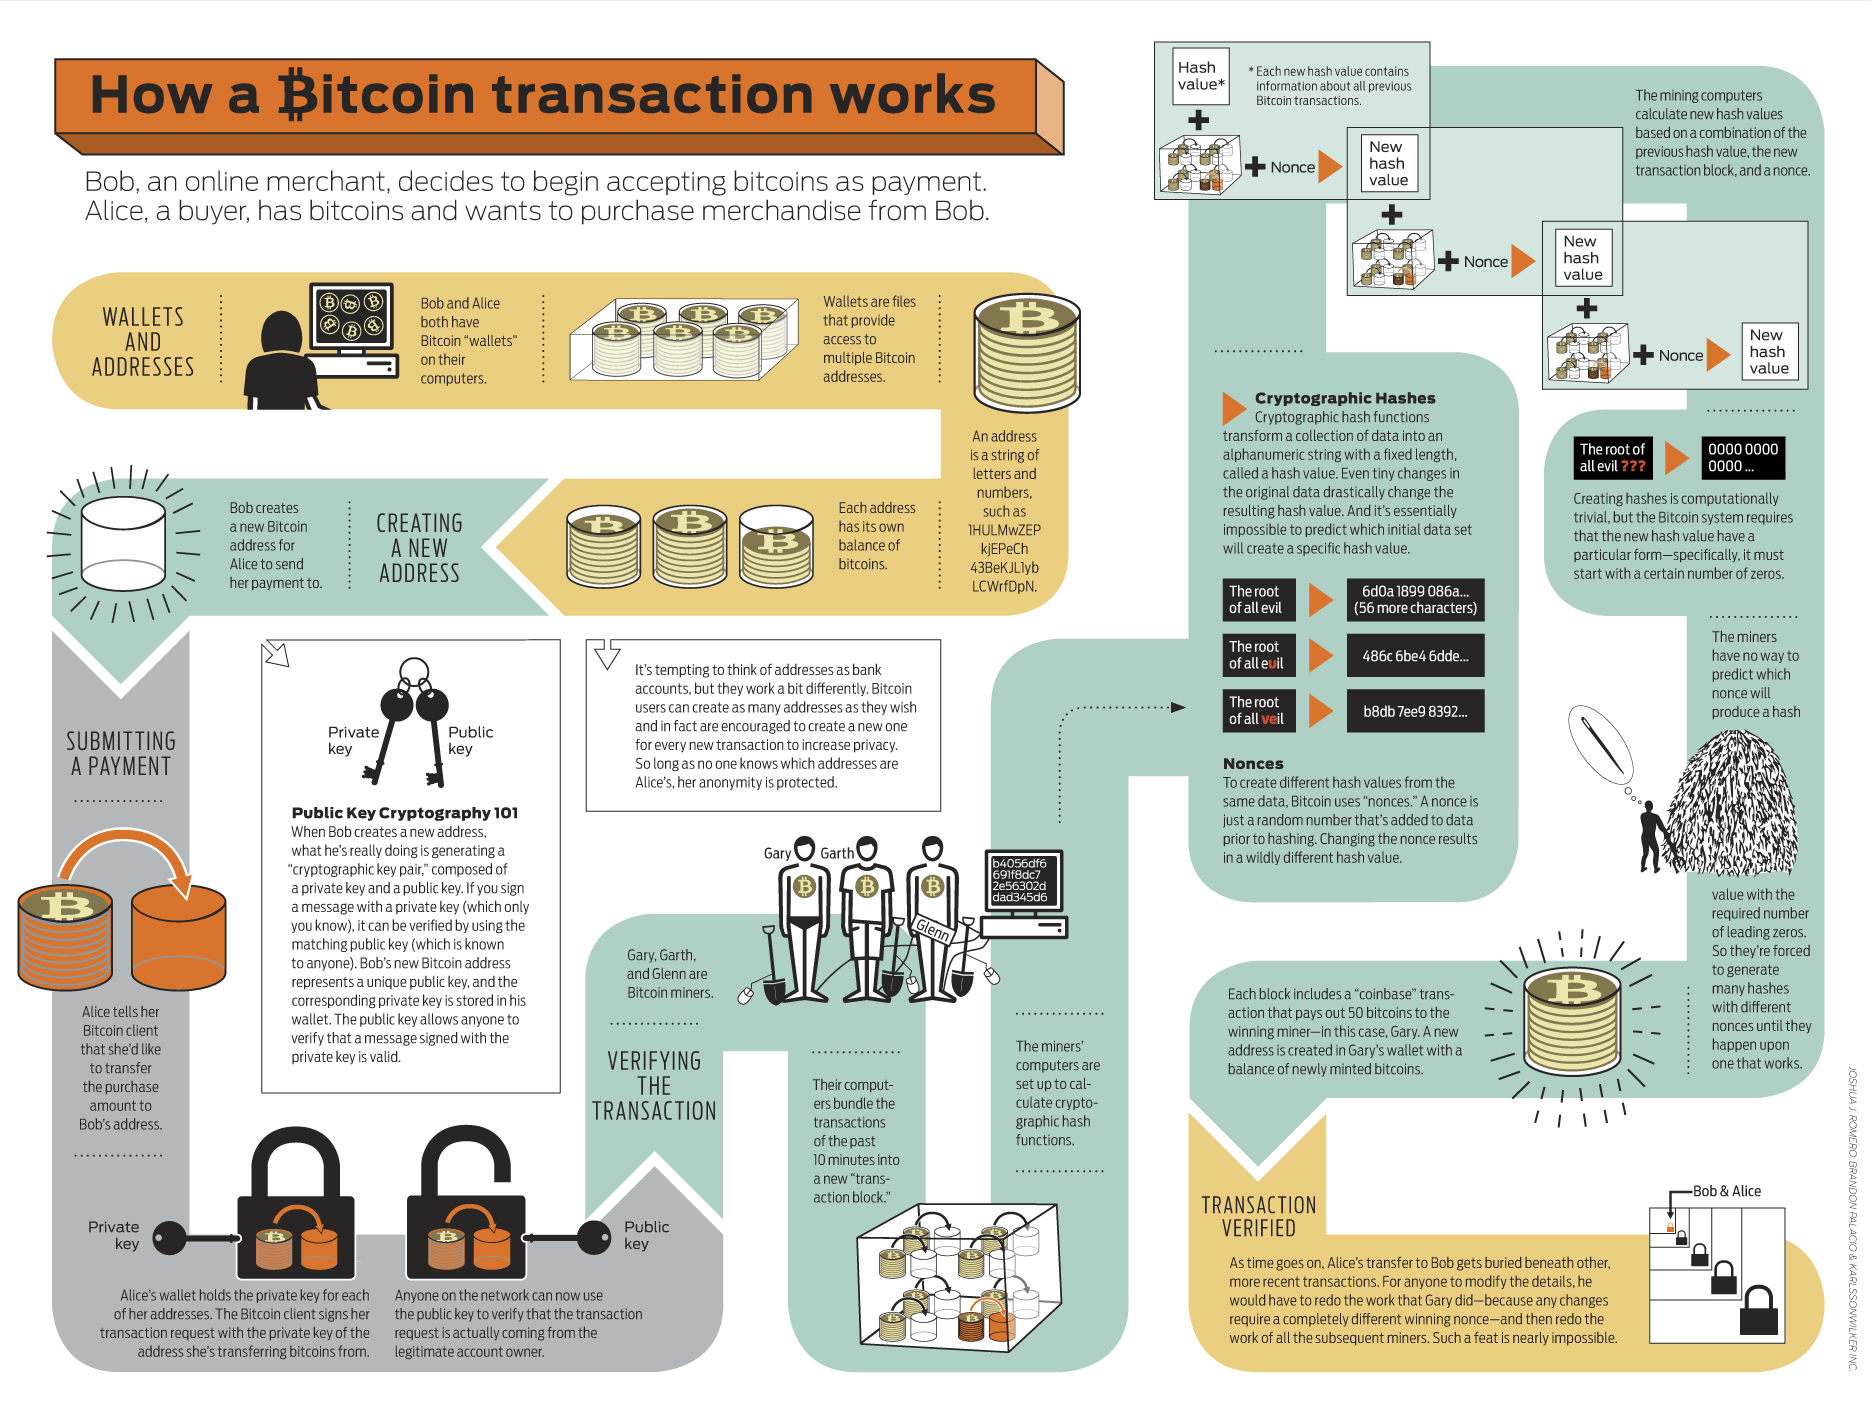
\includegraphics[scale=0.37]{images/how-a-bitcoin-transaction-works.jpg}
\end{frame}


\begin{frame}

	Děkuji za pozornost.

	\bigskip
	
	Doplňující otázky?

	\bigskip

	\bigskip

	\scriptsize
	Copyleft Karel Bílek, Ondřej Profant, 2013. Všechna práva vyhlazena. Sdílejte, upravujte a~nechte sdílet za stejných podmínek. 

	\bigskip

	Prezentace v~úplné formě\footnote{i se zdrojovými kódy} na:\\ 
	\url{https://www.github.com/kedrigern/prezentace-cs}.

	\bigskip

	Mail: ondrej.profant -at- pirati.cz 
\end{frame}

\end{document}
